The Liaison System is created to assure that the correct data collected from a microcontrollers is received correctly by the end user.
To achieve this, the system uses four equal but distinct microcontrollers, an internal voting system to assure that if any of the microcontrollers
disagree, it is marked as malfunctioning and is no longer allowed to send output. The output from the Liaison is extended with a system status
code that tells the end user if any of the microcontrollers are damaged, and the signal is then enhanced with an error correcting code such that
we can be more certain that the signal is not distorted on its way to the reciever.

\begin{figure}[h]
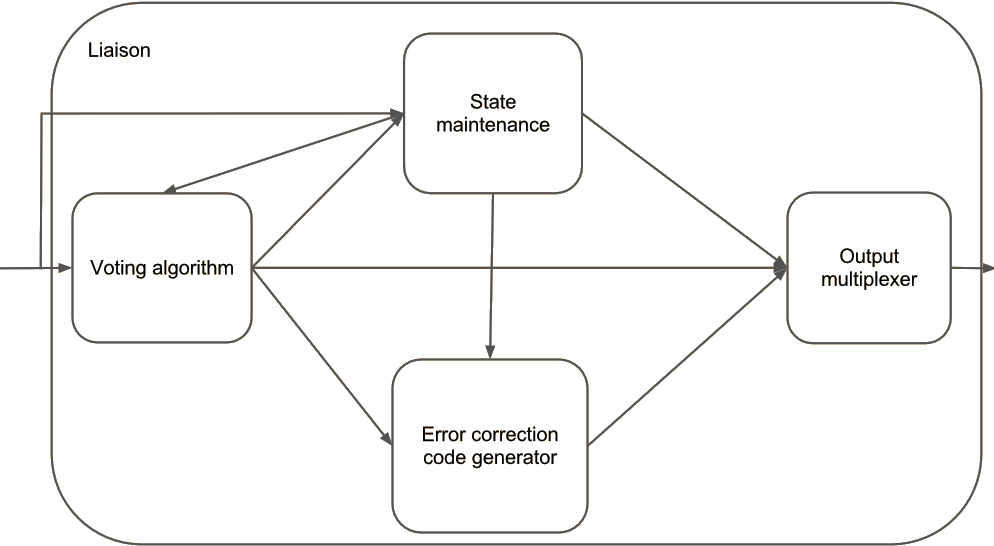
\includegraphics[width=15cm]{design/fig_overview}
\caption{Modules overview}
\label{fig:overview}
\end{figure}

As we can see from \autoref{fig:overview}, the internals of the Liaison can be modeled as four different pieces of hardware, each providing a
nessesary service to the system.

\subsection{Voting algorithm}
The system needs to distinguish between the working and the malfunctioning microcontrollers. To do this, the voting module knows what microcontrollers
that has shown sign of failure from earlier voting, and it needs to vote for the majority result of working microcontrollers. This modules
receives input directly from the microcontrollers, and it gets the current system state from the State Maintainance module.

\subsection{State maintainance}
The State Maintainance module is responsible for all internal states of the system. The system keeps track of what microcontrollers that can
no longer be trusted. This works by tagging those microcontrollers were the signal differs from the voted signal from the Voter module. When
a microcontroller has been tagged, the tag is not cleared until the entire system is reset.

This modules also outputs a system status vector as part of the Liaison output. This vector has one of four states as shown in \autoref{tbl:status}

\begin{table}[h]
        \centering
        \begin{tabular}{c|c|c}
        # Working MCUs     & System status & Bit-string \\
        \hline
        4 & Working        & 000 \\
        3 & Single failure & 001 \\
        2 & Double failure & 010 \\
        1 & System broken  & 111 \\
        0 & System broken  & 111
        \end{tabular}
        \caption{System Status}
        \label{tbl:status}
\end{table}

\subsection{Error Correcting Code Generator}
\subsection{Output mulitplexer}
